\section*{Introduction} % Why not just remove the * and have it add to content automatically?? -Agnes
\addcontentsline{toc}{section}{Introduction}
Principal Component Analysis is a method which aims at reducing the dimensionality of a dataset into a linearly uncorrelated set of features, each maximizing the variance on the observations.

The method presented here gather PCA and kernel methods by describing an efficient way to compute principal components in a feature space of large dimensionality that is related to the input space by a non-linear mapping. An illustration of this can be seen in Figure \ref{fig:kernel_pca}. This is achieved by the use of kernel functions similar to the ones used in Support Vector Machines (SVM). This report details how to achieve this basis transformation and apply it through a feature extraction based on a digit recognition experiment.

\begin{figure}[h!]
    \centering
    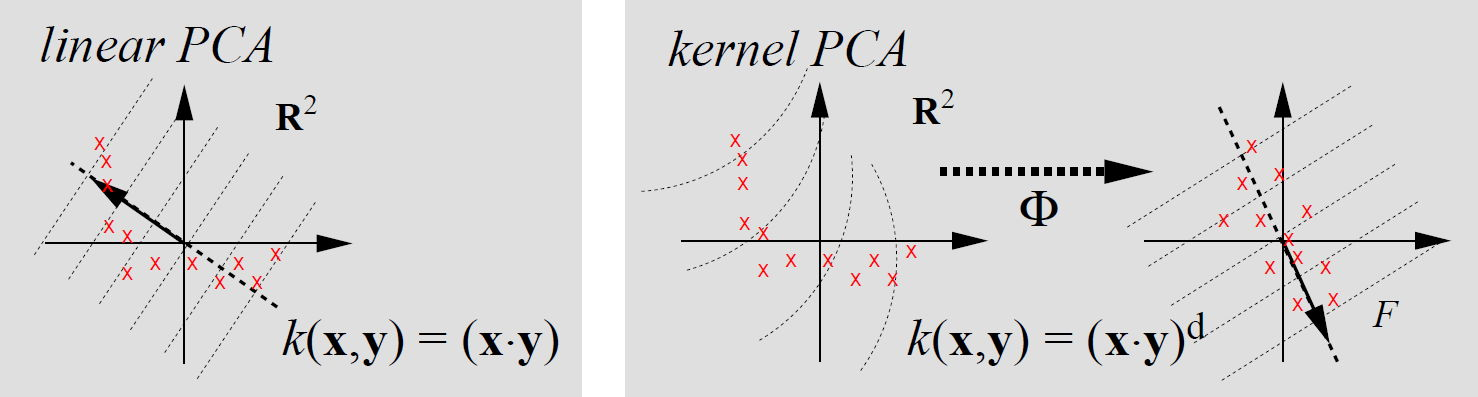
\includegraphics{img/kernel_pca.jpg}
    \caption{Comparison between linear PCA and kernel PCA}
    \label{fig:kernel_pca}
\end{figure}
